% ****** Start of file apssamp.tex ******
%
%   This file is part of the APS files in the REVTeX 4.1 distribution.
%   Version 4.1r of REVTeX, August 2010
%
%   Copyright (c) 2009, 2010 The American Physical Society.
%
%   See the REVTeX 4 README file for restrictions and more information.
%
% TeX'ing this file requires that you have AMS-LaTeX 2.0 installed
% as well as the rest of the prerequisites for REVTeX 4.1
%
% See the REVTeX 4 README file
% It also requires running BibTeX. The commands are as follows:
%
%  1)  latex apssamp.tex
%  2)  bibtex apssamp
%  3)  latex apssamp.tex
%  4)  latex apssamp.tex
%
\documentclass[%
 reprint,
%superscriptaddress,
%groupedaddress,
%unsortedaddress,
%runinaddress,
%frontmatterverbose, 
%preprint,
%showpacs,preprintnumbers,
%nofootinbib,
%nobibnotes,
%bibnotes,
 amsmath,amssymb,
 aps,
%pra,
%prb,
%rmp,
%prstab,
%prstper,
%floatfix,
]{revtex4-1}

\usepackage{graphicx}% Include figure files
\usepackage{dcolumn}% Align table columns on decimal point
\usepackage{bm}% bold math
%\usepackage{hyperref}% add hypertext capabilities
%\usepackage[mathlines]{lineno}% Enable numbering of text and display math
%\linenumbers\relax % Commence numbering lines

%\usepackage[showframe,%Uncomment any one of the following lines to test 
%%scale=0.7, marginratio={1:1, 2:3}, ignoreall,% default settings
%%text={7in,10in},centering,
%%margin=1.5in,
%%total={6.5in,8.75in}, top=1.2in, left=0.9in, includefoot,
%%height=10in,a5paper,hmargin={3cm,0.8in},
%]{geometry}

\begin{document}



\title{Homework 6}% Force line breaks with \\


\author{Hong Yao}
\author{Zhangjie Qin}
\affiliation{%
 Department of Physics, Virginia Tech, Blacksburg, VA 24060, USA }%
\date{\today}

\maketitle

%\tableofcontents

\section{Newton's theory of rainbow}
In this section, we will discuss the scattering of light from a spherical water drop. We will give the relation between the scattering angle and the impact parameter then calculate the scattering differential cross section. We will also calculate the angular width of the rainbow from red light to violet light.

\subsection{Relation between Scattering Angle and Impact Parameter}
\begin{figure}
    \centering
    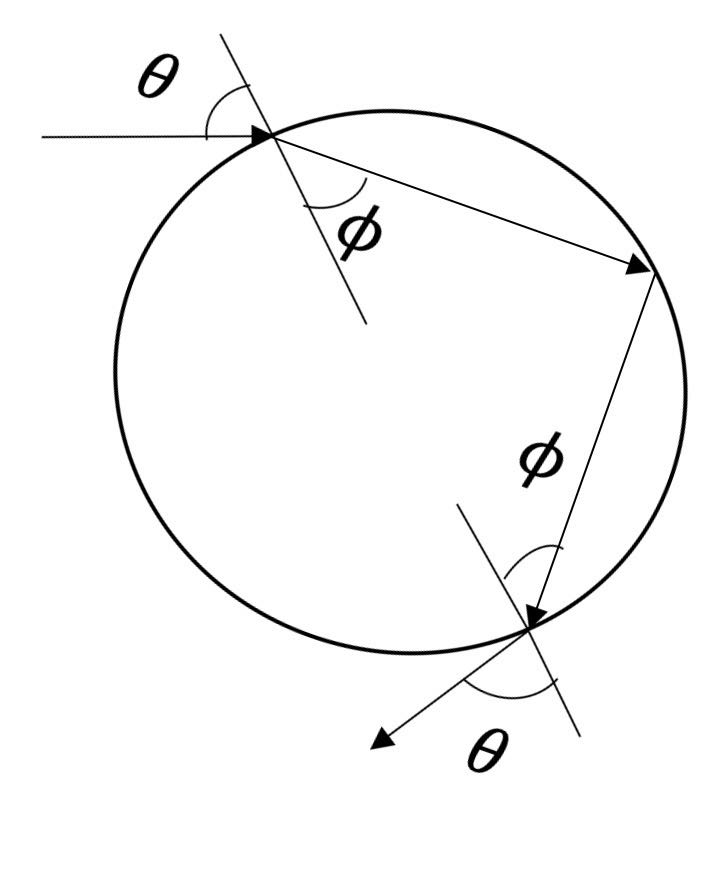
\includegraphics[scale=0.2]{optical.jpg}
    \caption{Optical Path of Single Reflection Scattering}
\end{figure}
\begin{figure}
    \centering
    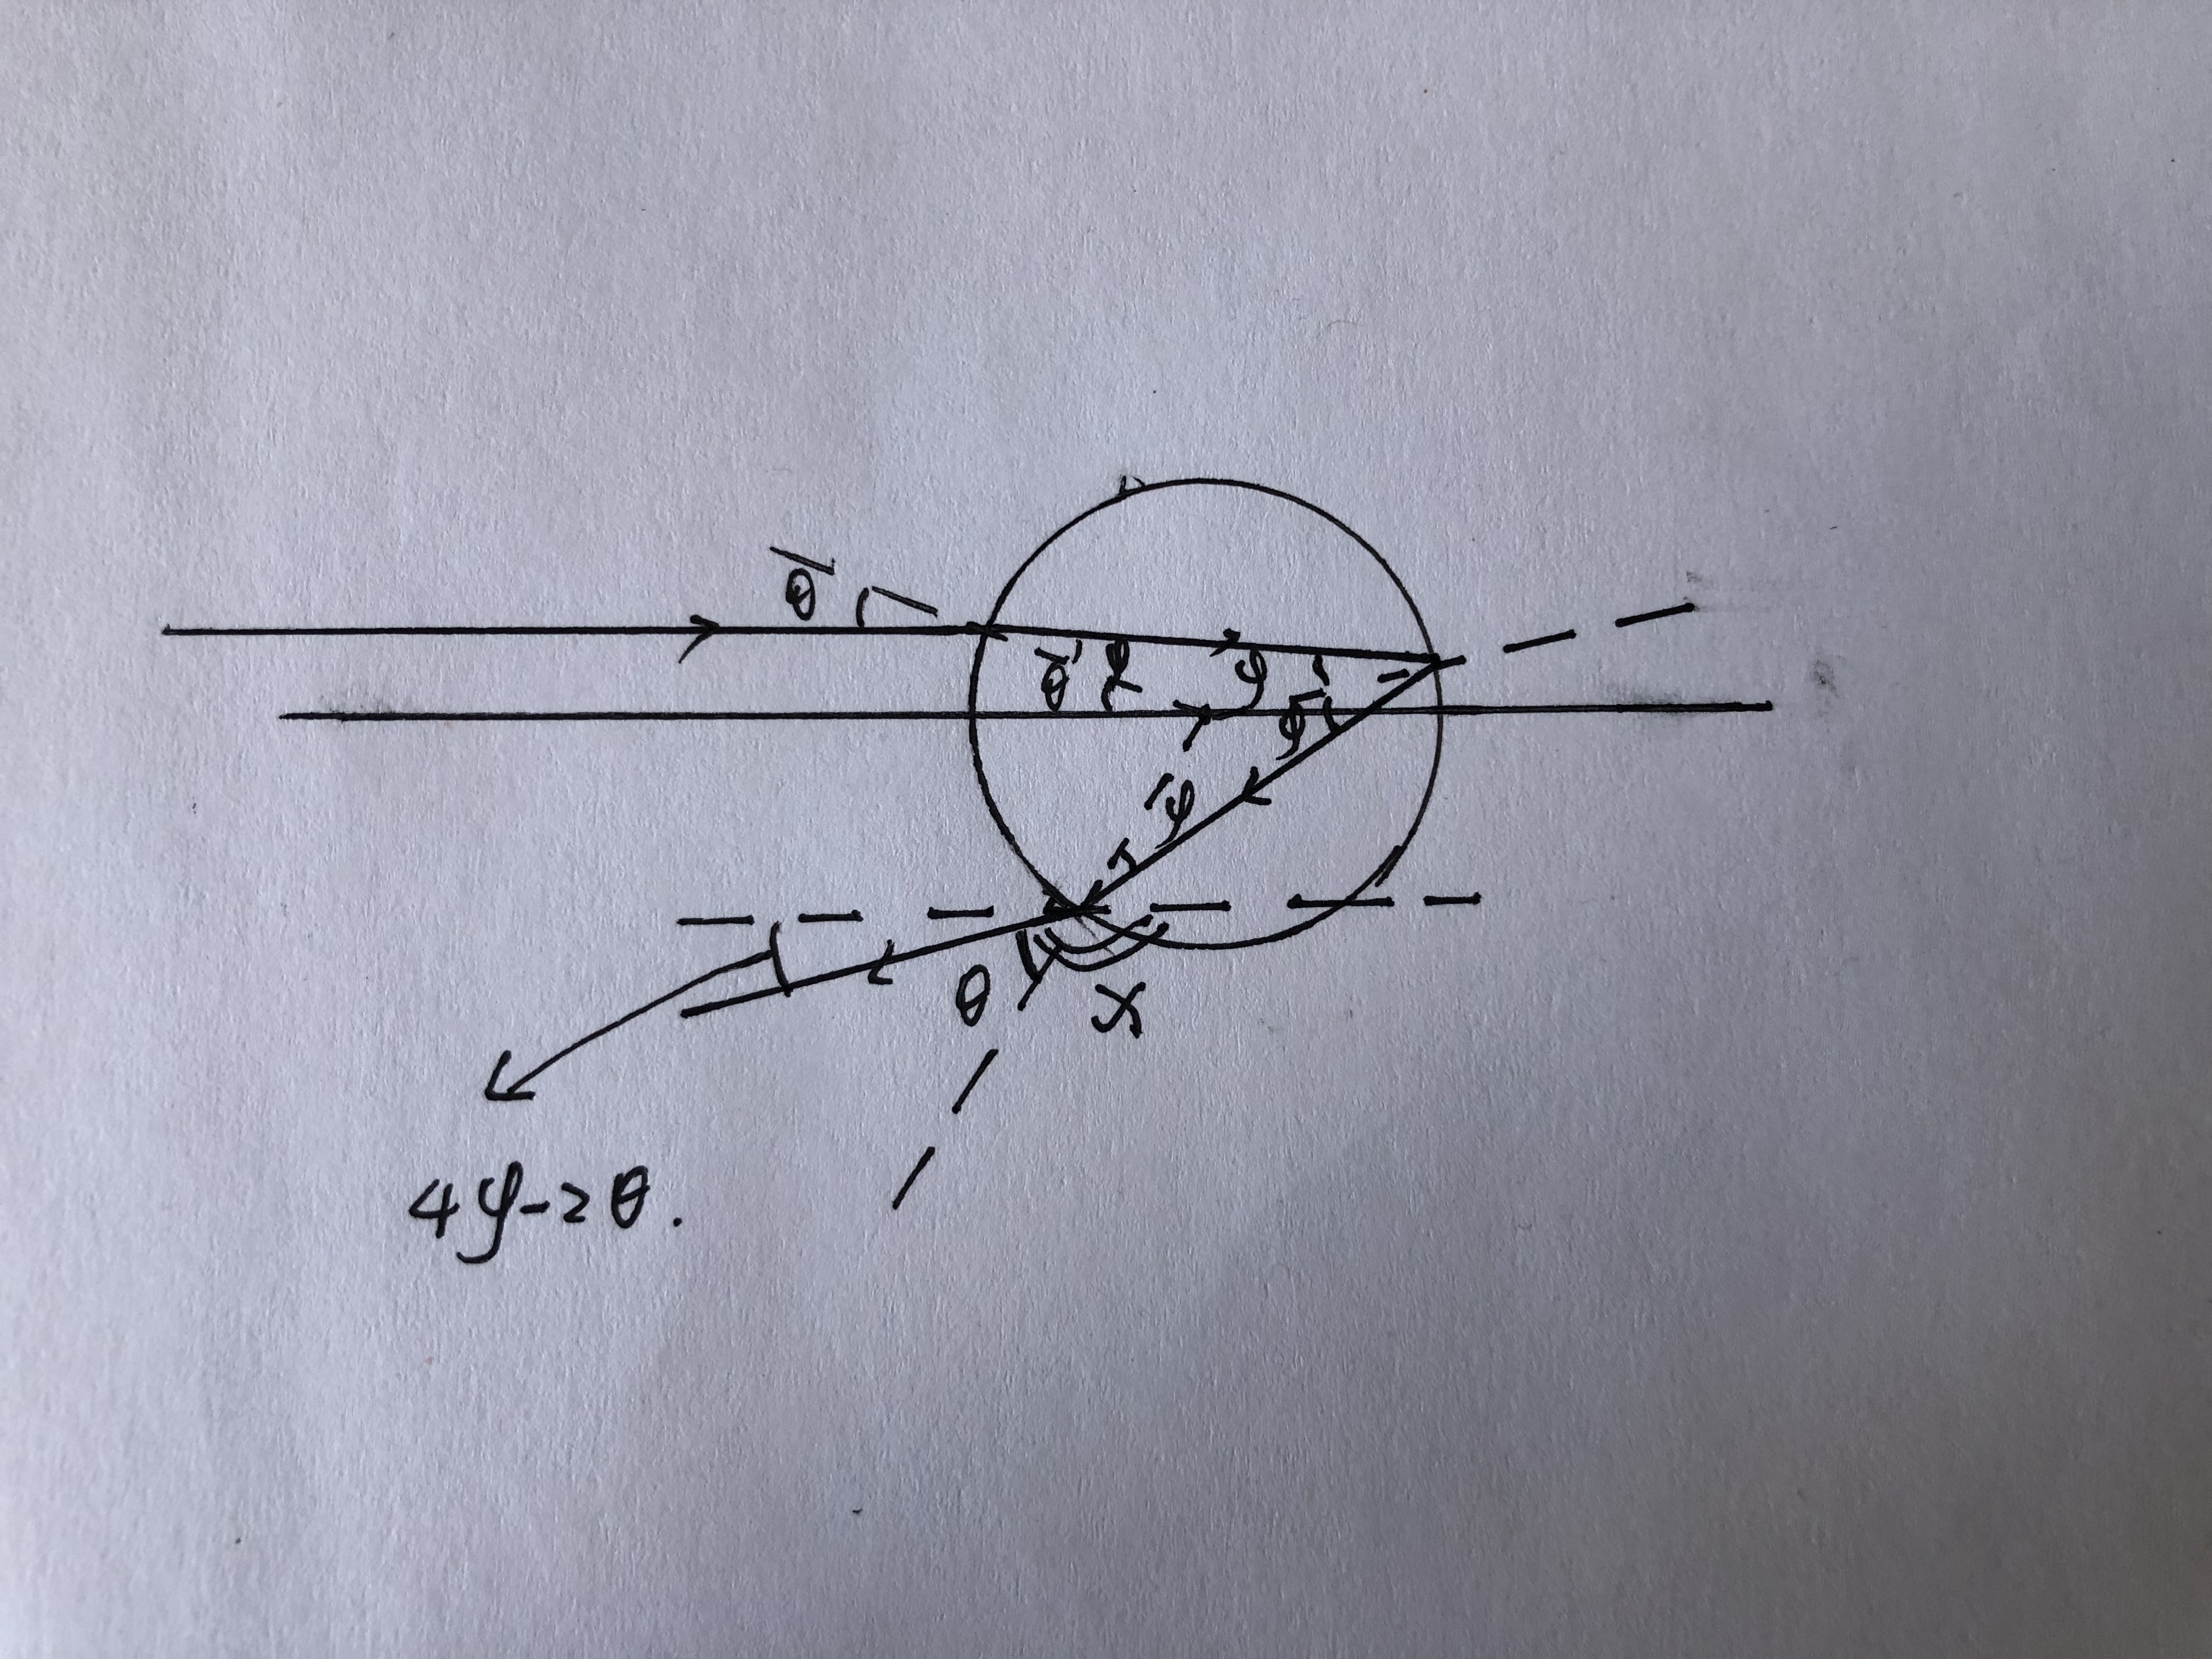
\includegraphics[scale=0.05]{geometryrelation.jpg}
    \caption{Geometry Relation between Angles}
    \label{fig:my_label}
\end{figure}
From the graph, it is easy to read that the scattering angle is
\begin{equation}
    \chi=\pi-4\phi+2\theta.
\end{equation}
where $\theta=\arcsin{b/R}$ is the incident angle and $\phi=\arcsin{b/(nr)}$ is the refraction angle.

From simple geometry, we can write down
\begin{equation}
\begin{aligned}
\phi&=\arcsin{\frac{b}{nR}}\\
\theta&=\arcsin{\frac{b}{R}}
\end{aligned}.
\end{equation}
From this relation, we can write $\chi$ as
\begin{equation}
    \chi=\pi-4\arcsin{\frac{b}{nR}}+2\arcsin{\frac{b}{R}}.
\label{scatteringangle}
\end{equation}
Since $n=\frac{4}{3}$, we can draw the relation between the scattering angle $\chi$ and impact parameter $b$ is showed in Fig.(\ref{chiandb}).
\begin{figure}
    \centering
    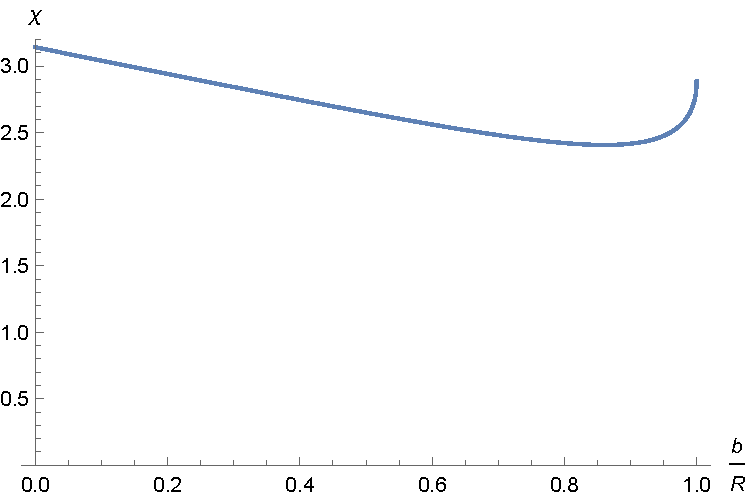
\includegraphics[scale=0.6]{scatteringanglevsb.pdf}
    \caption{Relation between scattering angle and impact parameter}
    \label{chiandb}
\end{figure}
From the figure, we can read that the function $b(\chi)$ of $\chi$ is a double-valued function.
\subsection{Differential Scattering Cross Section}
From the formula for the differential scattering cross section
\begin{equation}
    \frac{\mathrm{d}\sigma}{\mathrm{d}\Omega}=\frac{b}{\sin{\chi}}|\frac{\mathrm{d}b}{\mathrm{d}\chi}|.
\end{equation}
From Eq.(\ref{scatteringangle}), we finally get
\begin{equation}
    \frac{\mathrm{d}\sigma}{\mathrm{d}\Omega}=\frac{b}{\sin{[\chi(b)]}}\left|\frac{1}{\chi'(b)}\right|.
\label{crosssection}
\end{equation}
The relation between the differential scattering cross section and the impact parameter is showed in Fig.(\ref{diffcrosssection}).
\begin{figure}
    \centering
    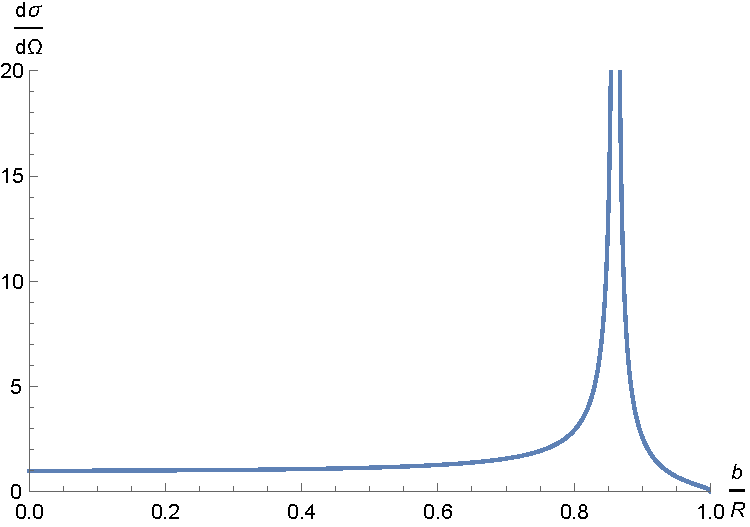
\includegraphics[scale=0.6]{diffcrosssecctionofb.pdf}
    \caption{Relation between $\frac{\mathrm{d}\sigma}{\mathrm{d}\Omega}$ and impact parameter}
    \label{diffcrosssection}
\end{figure}
From the parametric functions combined by Eq.(\ref{crosssection}) and Eq.(\ref{chiandb}), we can also find the relation between the scattering cross section and the scattering angle $\chi$, which is showed in Fig.(\ref{crosssectionofchi})
\begin{figure}
    \centering
    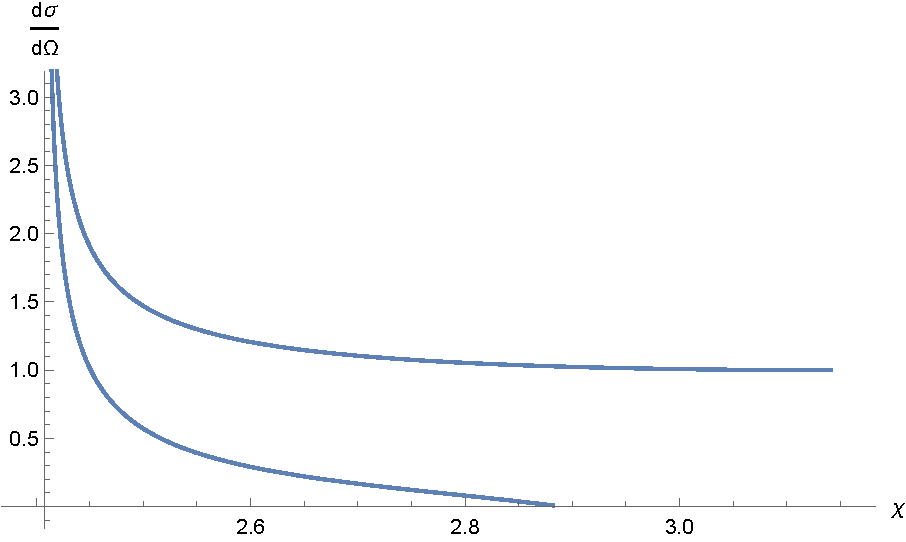
\includegraphics[scale=0.5]{crosssectionofchi.pdf}
    \caption{The relation between $\frac{\mathrm{d}\sigma}{\mathrm{d}\Omega}$ and $\chi$}
    \label{crosssectionofchi}
\end{figure}
It is a double-valued function due to the fact that the function $b(\chi)$ is a double-valued function. And the exact differential cross section is the sum of the two value at same $\chi$.
\subsection{The Width of the Rainbow}
Since the difference of the reflection index of red and violet light, we will have a rainbow. The reflection index for red and violet light are $n_r=1.332$ and $n_v=1.344$. Take these two valued into Eq.(\ref{scatteringangle}), we will get the relation between scattering angle and impact parameter for both red and violet light, which are showed in Fig.(\ref{redandviolet}).
\begin{figure}
    \centering
    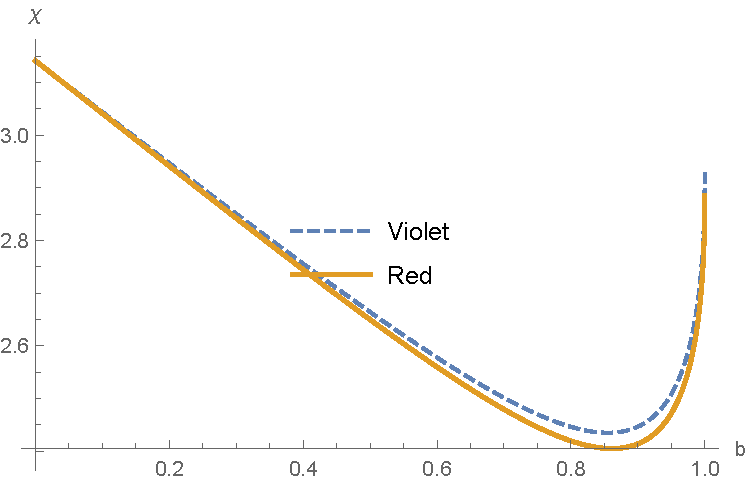
\includegraphics[scale=0.6]{redandviolet.pdf}
    \caption{Scattering Angle of Red and Violet Light}
    \label{redandviolet}
\end{figure}
We can also find the angle width between red and violet light as a function of the impact parameter, which is showed in Fig.(\ref{anglewidth}). And the maximum angle width is around $0.04$.
\begin{figure}
    \centering
    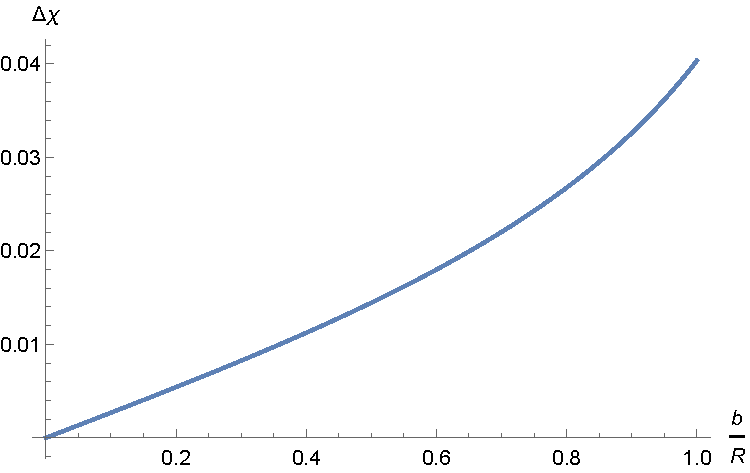
\includegraphics[scale=0.6]{anglewidth.pdf}
    \caption{The Angle Width versus Impact Parameter}
    \label{anglewidth}
\end{figure}
\subsection{Double Scattering}
\begin{figure}
    \centering
    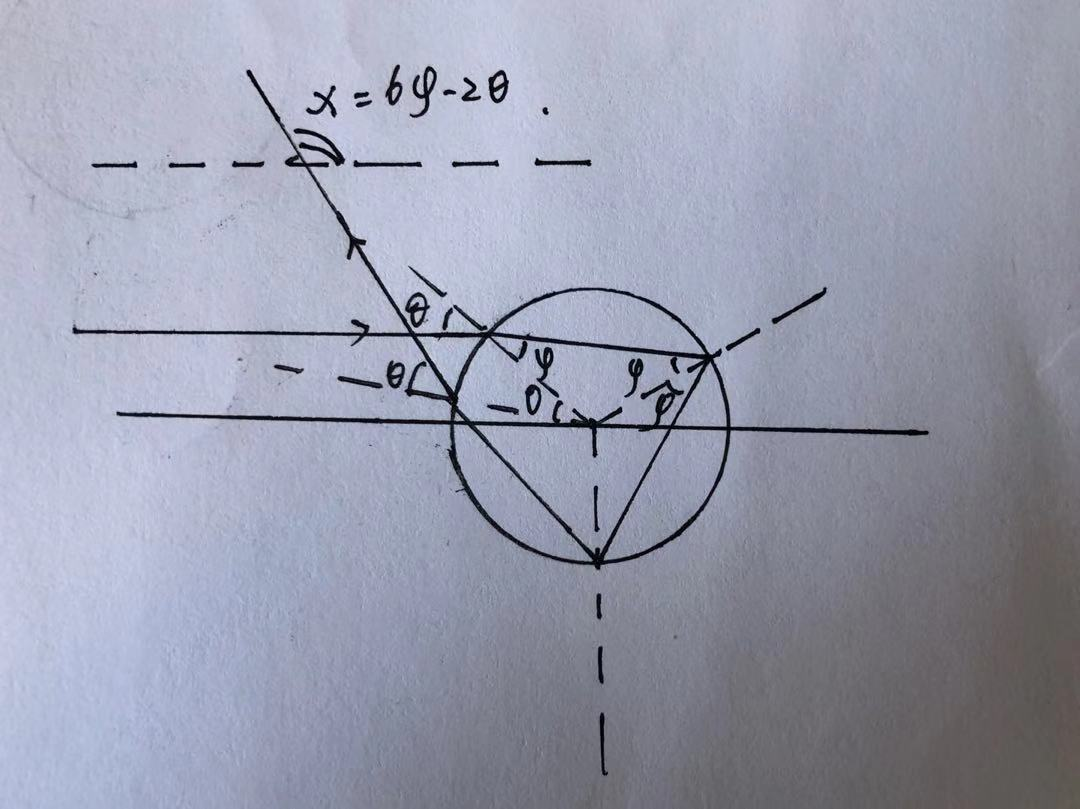
\includegraphics[scale=0.2]{geometryrelationdouble.jpg}
    \caption{Geometry Relation for Double Scattering}
    \label{fig:my_label}
\end{figure}
It is trivial from the geometry that the scattering angle is
\begin{equation}
    \chi=6\phi-2\theta=6\arcsin{\frac{b}{nR}}-2\arcsin{\frac{b}{R}},
\end{equation}
which is showed in Fig.(\ref{doubelangle}).
\begin{figure}
    \centering
    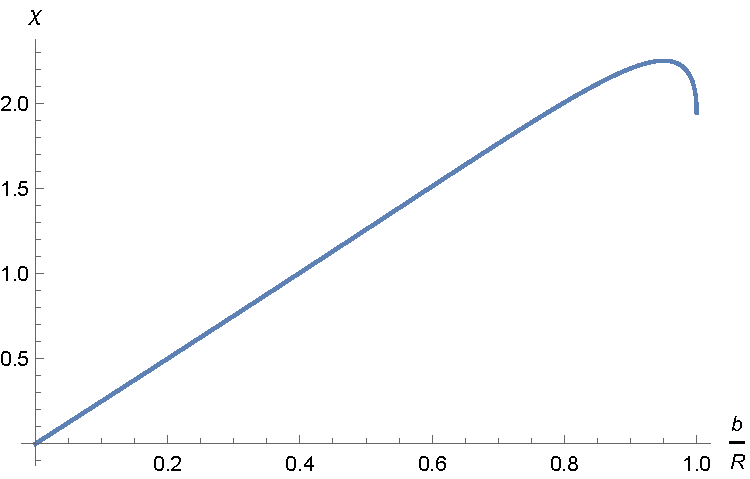
\includegraphics[scale=0.6]{scatteringanlgeofdouble.pdf}
    \caption{Scattering Angle of Double Reflection}
    \label{doubelangle}
\end{figure}

We can also calculate the scattering cross section from Eq.(\ref{crosssection}), which is showed in Fig.(\ref{doubleparameter}) and Fig.(\ref{doubelangle}). The function of the differential cross section about the scattering angle is still a double-valued function and the real cross section would be the sum of the two values.
\begin{figure}
    \centering
    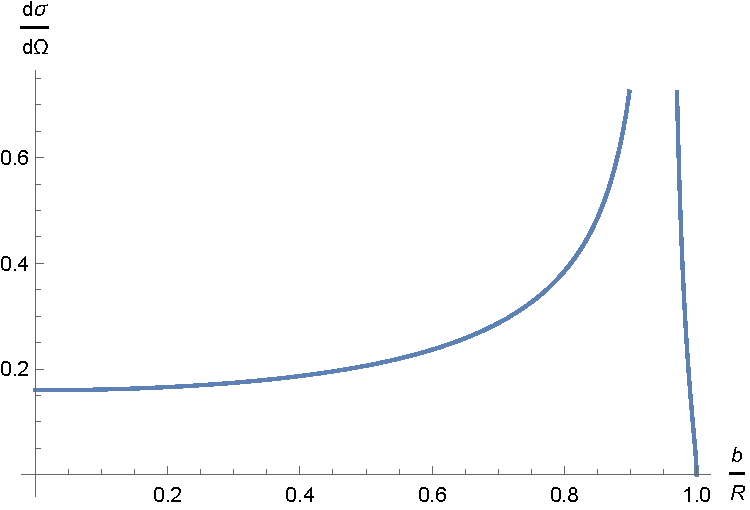
\includegraphics[scale=0.6]{crosssectiondouble.pdf}
    \caption{Cross Section versus Impact Parameter}
    \label{doubleparameter}
\end{figure}
\begin{figure}
    \centering
    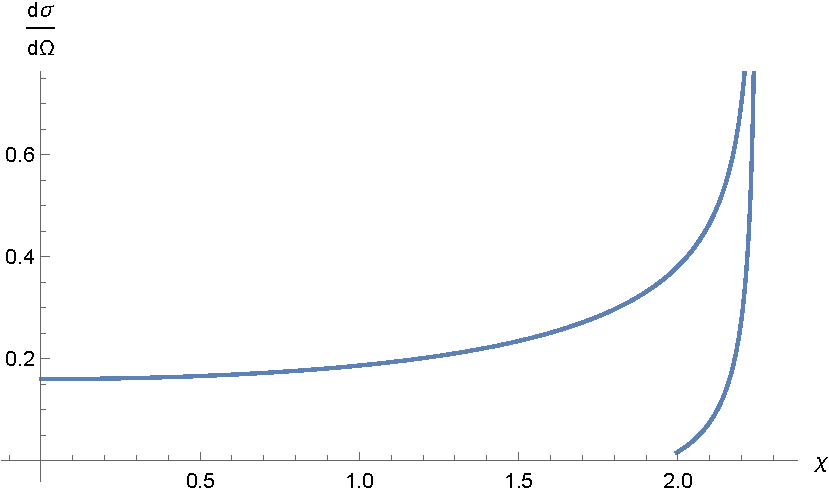
\includegraphics[scale=0.6]{crossectiondoubleofchi.pdf}
    \caption{Cross Section Versus Scattering Angle}
    \label{doubleangle}
\end{figure}

We can also calculate the angle width of the rainbow for double reflection scattering. The scattering angle for red and violet light are showed in Fig.(\ref{doublerednandviolet}).
\begin{figure}
    \centering
    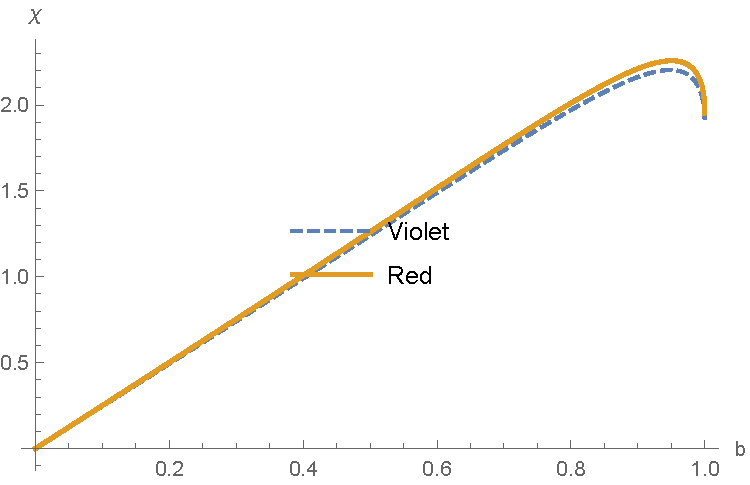
\includegraphics[scale=0.6]{redandvioletdouble.pdf}
    \caption{Scattering Angle of Red and Violet Light for Double Reflection}
    \label{doublerednandviolet}
\end{figure}
We can also calculate the angle width which is showed in Fig.(\ref{doubleanglewidth}). The maximum angle width is $0.06$.

\begin{figure}
    \centering
    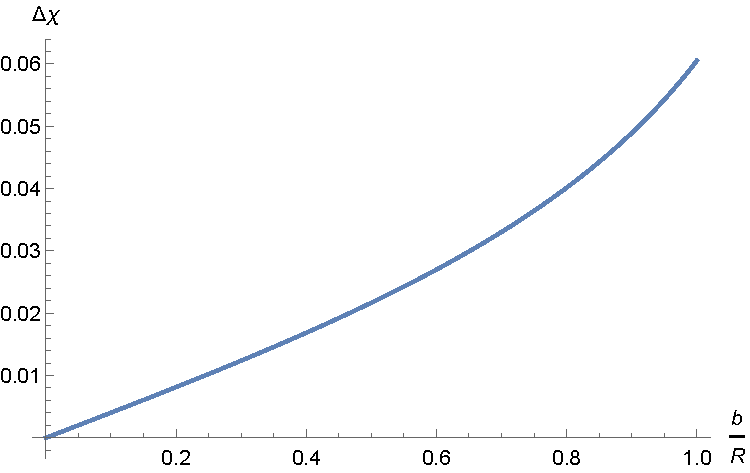
\includegraphics[scale=0.6]{doubleanglewidth.pdf}
    \caption{The Angle Width for Double Reflection Scattering}
    \label{doubleanglewidth}
\end{figure}





\section{Noether's Theorem for Particle Dynamics}
In this section, we discuss the Noether's theorem for particle dynamics. We give the general formula of Noether's Theorem and then give the conservation law of momentum, angular momentum and energy seperately.
\subsection{Noether's Theorem}
We have the Lagrangian for a particle as
\begin{equation}
    L=L(\vec{q},\dot{\vec{q}},t).
\end{equation}
We make the variation of the Lagrangian
\begin{equation}
    \delta L=(\frac{\partial L}{\partial \vec{q}}-\frac{\mathrm{d}}{\mathrm{d}t}\frac{\partial L}{\partial\dot{\vec{q}}})\cdot\delta\vec{q}+\frac{\mathrm{d}}{\mathrm{d}t}(\frac{\partial L}{\partial \dot{\vec{q}}}\cdot\delta\vec{q}).
\end{equation}
From the Euler-Lagrange Equation, we know the first term on RHS is $0$. thus, we have
\begin{equation}
    \frac{\mathrm{d}}{\mathrm{d}t}(\frac{\partial L}{\partial \dot{\vec{q}}}\cdot\delta\vec{q})-\delta L=0
    \label{beforenoether}
\end{equation}
Term $\delta L$ can always been written as $\frac{\mathrm{d}}{\mathrm{d}t}F$, where $F$ is a function of $\vec{q}$, $\dot{\vec{q}}$ and $t$. Thus, Eq.(\ref{beforenoether}) can be written as
\begin{equation}
    \frac{\mathrm{d}}{\mathrm{d}t}(\frac{\partial L}{\partial \dot{\vec{q}}}\cdot\delta\vec{q}-F)=0.
\label{noether'stheorem}
\end{equation}
It is obvious that $(\frac{\partial L}{\partial \dot{\vec{q}}}\cdot\delta\vec{q}-F)$ is a conserved charge.
\subsection{Conservation Law of Momentum}
We have the Lagrangian for free particle
\begin{equation}
    L=\frac{1}{2}m\dot{\vec{x}}^2.
\label{lagrangian}
\end{equation}
When we add the variation on spatial coordinate $\vec{x}\rightarrow\vec{x}+\delta\vec{x}$, we have
\begin{equation}
\begin{aligned}
    \frac{\partial L}{\partial\dot{\vec{x}}}&=m\dot{\vec{x}}
    \\\delta L&=\delta\vec{x}\frac{\mathrm{d}}{\mathrm{d}x}L=0
\end{aligned}
\label{variationofposition}
\end{equation}
Take Eq.(\ref{variationofposition}) into Eq.(\ref{noether'stheorem}), we can get
\begin{equation}
    \frac{\mathrm{d}}{\mathrm{d}t}(m\dot{\vec{x}}\cdot\delta\vec{x})=0.
\end{equation}
Since the variation $\delta\vec{x}$ is arbitrary and time-independent, we have
\begin{equation}
    \frac{\mathrm{d}}{\mathrm{d}t}(m\dot{\vec{x}})=0.
\end{equation}
This is the conservation law of momentum and $\vec{p}=m\dot{\vec{x}}$ is the momentum of the free particle.
\subsection{Conservation Law of Angular Momentum}
We have the Lagrangian for free particle from Eq.(\ref{lagrangian}),
\begin{equation}
    L=\frac{1}{2}m\dot{\vec{x}}^2=\frac{1}{2}mx_ix^i.
\end{equation}
where $i=1,2,3$ and the above equation follows Einstein's summation rule.
Consider we have a rotation $x_i\rightarrow\Lambda_i^jx_j$. Where the rotation is infinitisimal, we have 
\begin{equation}
    \Lambda_i^j=\delta_i^j+\omega_i^j,
\end{equation}
where matrix $\omega$ is anti-symmetric.

Thus, we have
\begin{equation}
\begin{aligned}
    \frac{\partial L}{\partial \dot{x}_i}&=m\dot{x}^i
    \\\delta x_i&=\omega_i^jx_j
    \\\delta L&=0
\end{aligned}
\label{variationofangle}
\end{equation}
Take Eq.(\ref{variationofangle}) into Eq.(\ref{noether'stheorem}), we have
\begin{equation}
    \frac{\mathrm{d}}{\mathrm{d}t}(m\dot{x}^ix_j\omega_i^j)=0.
\end{equation}
Since $\omega_i^j$ is anti-symmetric and time-independent, we have
\begin{equation}
    \frac{\mathrm{d}}{\mathrm{d}t}(m\dot{x}_jx_i-m\dot{x}_ix_j)=0.
\end{equation}
This is the conservation law of angular momentum and $L_k=\epsilon_{ijk}(m\dot{x}_jx_i-m\dot{x}_ix_j)$ is the $k$-th conponent of angular momentum.
\subsection{Conservation Law of Energy}
We have the Lagrangian for the particle
\begin{equation}
    L=\frac{1}{2}m\dot{\vec{x}}^2-V(\vec{x}).
\end{equation}
When we add a variation of time that $t\rightarrow t+\delta t$, we will have
\begin{equation}
\begin{aligned}
    \delta\vec{x}&=\delta t\frac{\mathrm{d}}{\mathrm{d}t}\vec{x}
    \\\delta L&=\delta t\frac{\mathrm{d}}{\mathrm{d}t}L
    \\\frac{\partial L}{\partial \dot{\vec{x}}}&=m\dot{\vec{x}}
\end{aligned}
\label{variationoftime}
\end{equation}
Take Eq.(\ref{variationoftime}) into Eq.(\ref{noether'stheorem}), we will obtain
\begin{equation}
    \frac{\mathrm{d}}{\mathrm{d}t}(\frac{1}{2}m\dot{\vec{x}}^2+V(\vec{x}))=0.
\end{equation}
This is the conservation law of energy and $E=\frac{1}{2}m\dot{\vec{x}}^2+V(\vec{x})$ is the energy for the particle.
\end{document}
%
% ****** End of file apssamp.tex ******